\documentclass[draft,caption=numbered]{beamer}
\usetheme[color=screen]{UniBern}

%\setbeameroption{show notes}

\usepackage{lmodern}
\usepackage[english]{babel}
\usepackage{microtype}
\usepackage{textcomp}
\usepackage[backend=biber, style=alphabetic, url=false]{biblatex}
\addbibresource{../../Documents/library.bib}
\usepackage{graphicx}
\usepackage{caption}
    \captionsetup[figure]{labelformat=empty} % No 'figure' in figures
\usepackage{tikz}
	\usetikzlibrary{spy}
\usepackage[detect-all=true]{siunitx}
\usepackage{csquotes}
\usepackage{animate}
\usepackage{booktabs}
\usepackage[absolute,overlay]{textpos} %for the \source{} command
\usepackage{gitinfo2}
\usepackage{xspace}
\usepackage{hyperref}

\hypersetup{pdfstartview={Fit}}
\setbeamertemplate{caption}{\insertcaption}
\setbeamertemplate{caption}[numbered]

\newcommand{\imsize}{\linewidth}
\newlength\imagewidth % needed for scalebars
\newlength\imagescale % ditto
\newcommand{\uct}{\si{\micro}CT\xspace}
\newcommand{\uaf}{\si{\micro}AngioFil\xspace}

\newcommand{\source}[1]{%http://tex.stackexchange.com/a/48485/828
    \begin{textblock*}{4cm}(8.7cm,8.6cm)%
    \begin{beamercolorbox}[ht=0.5cm,right]{framesource}%
    \tiny\usebeamerfont{framesource}\usebeamercolor[fg]{framesource} Source: {#1}%
    \end{beamercolorbox}%
    \end{textblock*}%
}

% Biblatex: http://tex.stackexchange.com/a/13076/828
% % Format bibliography for beamer
% % http://tex.stackexchange.com/a/10686/828
% \renewbibmacro{in:}{}
% % http://tex.stackexchange.com/a/13076/828
% \AtEveryBibitem{\clearfield{title}}
% \AtEveryBibitem{\clearfield{journaltitle}}
% \AtEveryBibitem{\clearfield{year}}
% \AtEveryBibitem{\clearfield{pages}}
% \AtEveryBibitem{\clearfield{volume}}
% \AtEveryBibitem{\clearfield{number}}
% %http://tex.stackexchange.com/a/40710/828
% \usepackage{xpatch}
% \xpatchbibmacro{month}{%
%   \printtext[parens]%
% }{%
%   \setunit*{\addperiod\space}%
%   \printtext%
% }{}{} 

\subtitle{Several examples as well as details in lung and brain imaging}
\author[David Haberthür]{David Haberthür \and\tiny Adolfo Odriozola \and Ruslan Hlushchuk \and Valentin Djonov}
\institute{Institute of Anatomy\\Universität Bern}
\date{February 9, 2017\\Internal seminar@Institute of Anatomy}

%\useoutertheme{split}

\begin{document}
\title[\si{\micro}CT in biological studies]{\si{\micro}CT-imaging at the Institute of Anatomy} % http://tex.stackexchange.com/a/144445/828

\defbeamertemplate{footline}{unibe}
{%
	\usebeamercolor[fg]{page number in head/foot}%
	\usebeamerfont{page number in head/foot}%
	\hspace*{\fill}%
	\insertshortauthor%
	\hspace*{\fill}%|\hspace*{\fill}%
	\insertshorttitle%
	\hspace*{\fill}%|\hspace*{\fill}%
	v.~\gitAbbrevHash%
	\hspace*{\fill}%|\hspace*{\fill}%
	\insertframenumber\,/\,\insertpresentationendpage%
	\hspace*{\fill}%
	\vskip2pt%
}
\setbeamertemplate{footline}[unibe]

{
\setbeamertemplate{footline}{} % http://tex.stackexchange.com/a/18829/828
\begin{frame}
  \titlepage
\end{frame}
}
\addtocounter{framenumber}{1}

\begin{frame}{Contents}
	\tableofcontents
\end{frame}

\section{Overview}
\begin{frame}{Backstory}
    \begin{itemize}
        \item Lung fibrosis grading \cite{Ashcroft1988a}
        \item \emph{Correct} sampling for proper assessment
        \item \uct is a tool to help grade fibrosis
        \begin{itemize}
            \item Detect and grade fibrosis
            \item Get indications where to perform the sampling
        \end{itemize}
        \item Cancer metastasis (\SI{2}{year} after radiation treatment fibrosis is induced)
        \item Cancer treatment
        \begin{itemize}
            \item Antiangiogenesis (failed)
            \item Radiation therapy, namely MRT \cite{Bronnimann2016} (probably better citation needed)!
        \end{itemize}
    \end{itemize}
\end{frame}

\begin{frame}{Stories}
    \begin{itemize}
        \item  Overview of metastatis (Ochsenbein sample)
        \item Fibrosis grading (3View/uCT)
        \item Grenoble brains, assessing different parameters `easily'.
    \end{itemize}
\end{frame}

\section{(\si{\micro})CT}
\renewcommand{\imsize}{0.618\linewidth}
\begin{frame}{CT in theory}
    \begin{figure}[h]
    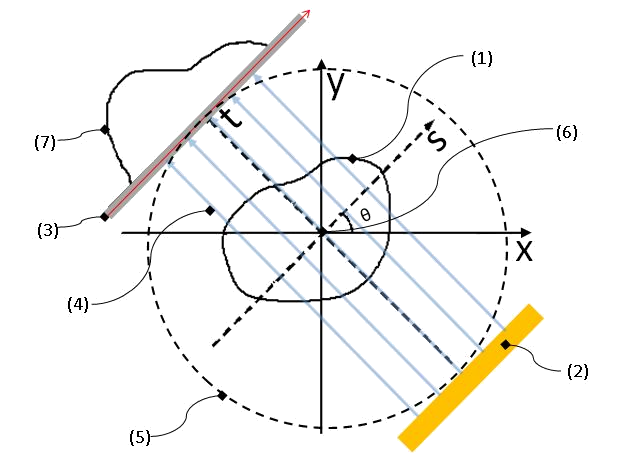
\includegraphics[width=\imsize]{img/CT_PRINCI_PB}
    \caption[CT]{Parallel beam CT.\\
        1: Object
        2: Parallel beam light source
        3: Screen
        4: Transmitted beam\\
        5: Datum circle
        6: Origin
        7: 1D image}
    \end{figure}
    \source{\href{https://commons.wikimedia.org/wiki/File:CT_PRINCI_PB.jpg}{enwp.org/tomography}}
\end{frame}

\section{Several examples}
\begin{frame}{Zebrafish}
    \renewcommand{\imsize}{\linewidth}%
    \begin{figure}%
        \pgfmathsetlength{\imagewidth}{\imsize}%
        \pgfmathsetlength{\imagescale}{\imagewidth/1651}%
        \def\x{1020}% scalebar-x starting at golden ratio of image width of 1651px = 1020
        \def\y{391}% scalebar-y at 90% of image height of 434px = 391
        \begin{tikzpicture}[x=\imagescale,y=-\imagescale]%
            \node[anchor=north west, inner sep=0pt, outer sep=0pt] at (0,0) {\includegraphics[width=\imagewidth]{img/{{zebrafish_rec_voi_side}}}};
            % 1615px = 35.48 > 100px = 2198um > 23px = 500um, 5px = 100um
            %\draw[|-|,blue,thick] (20,154) -- (1634,127) node [sloped,midway,above,fill=white,semitransparent,text opacity=1] {\SI{35.487480000000005}{\milli\meter} (1615px) TEMPORARY!};
            \draw[|-|] (\x,\y) -- (\x+234.19,\y) node [midway,above] {\SI{5}{\milli\meter}};
        \end{tikzpicture}%
        \caption{Visualization of a tomographic scan of a zebrafish, fixed in \SI{4}{\percent} PFA.}%
    \end{figure}%
\end{frame}

\begin{frame}{Rat head}
    \renewcommand{\imsize}{0.9\linewidth}%
    \begin{figure}%
        \pgfmathsetlength{\imagewidth}{\imsize}%
        \pgfmathsetlength{\imagescale}{\imagewidth/1400}%
        \def\x{865}% scalebar-x starting at golden ratio of image width of 1400px = 865
        \def\y{560}% scalebar-y at 90% of image height of 622px = 560
        \def\mag{4}    % magnification of inset
        \begin{tikzpicture}[x=\imagescale,y=-\imagescale]
            \node[anchor=north west, inner sep=0pt, outer sep=0pt] at (0,0) {\includegraphics[width=\imagewidth]{./img/{{ratwholehead_rec_side}}}};
            %\spy [red] on (1100,322) in node at (0,0) [anchor=north west];
            % 1358px = 47.76mm > 100px = 3517um > 14px = 500um, 3px = 100um
            %\draw[|-|,blue,thick] (23,291) -- (1380,311) node [sloped,midway,above,fill=white,semitransparent,text opacity=1] {\SI{47.76}{\milli\meter} (1358px) TEMPORARY!};
            \draw[|-|] (\x,\y) -- (\x+140,\y) node [midway,above] {\SI{5}{\milli\meter}};
        \end{tikzpicture}%
        \caption{Visualization of a tomographic scan of a rat head, instilled with \uaf and fixed in \SI{4}{\percent} PFA.}%
    \end{figure}%
\end{frame}

\begin{frame}{Spider}
\end{frame}

\begin{frame}{Rat brain vessels}
	\renewcommand{\imsize}{0.7\linewidth}%
    \begin{figure}%
        \pgfmathsetlength{\imagewidth}{\imsize}%
        \pgfmathsetlength{\imagescale}{\imagewidth/1950}%
        \def\x{1205}% scalebar-x starting at golden ratio of image width of 1950px = 1205
        \def\y{1230}% scalebar-y at 90% of image height of 1367px = 1230
        \begin{tikzpicture}[x=\imagescale,y=-\imagescale]
            \node[anchor=north west, inner sep=0pt, outer sep=0pt] at (0,0) {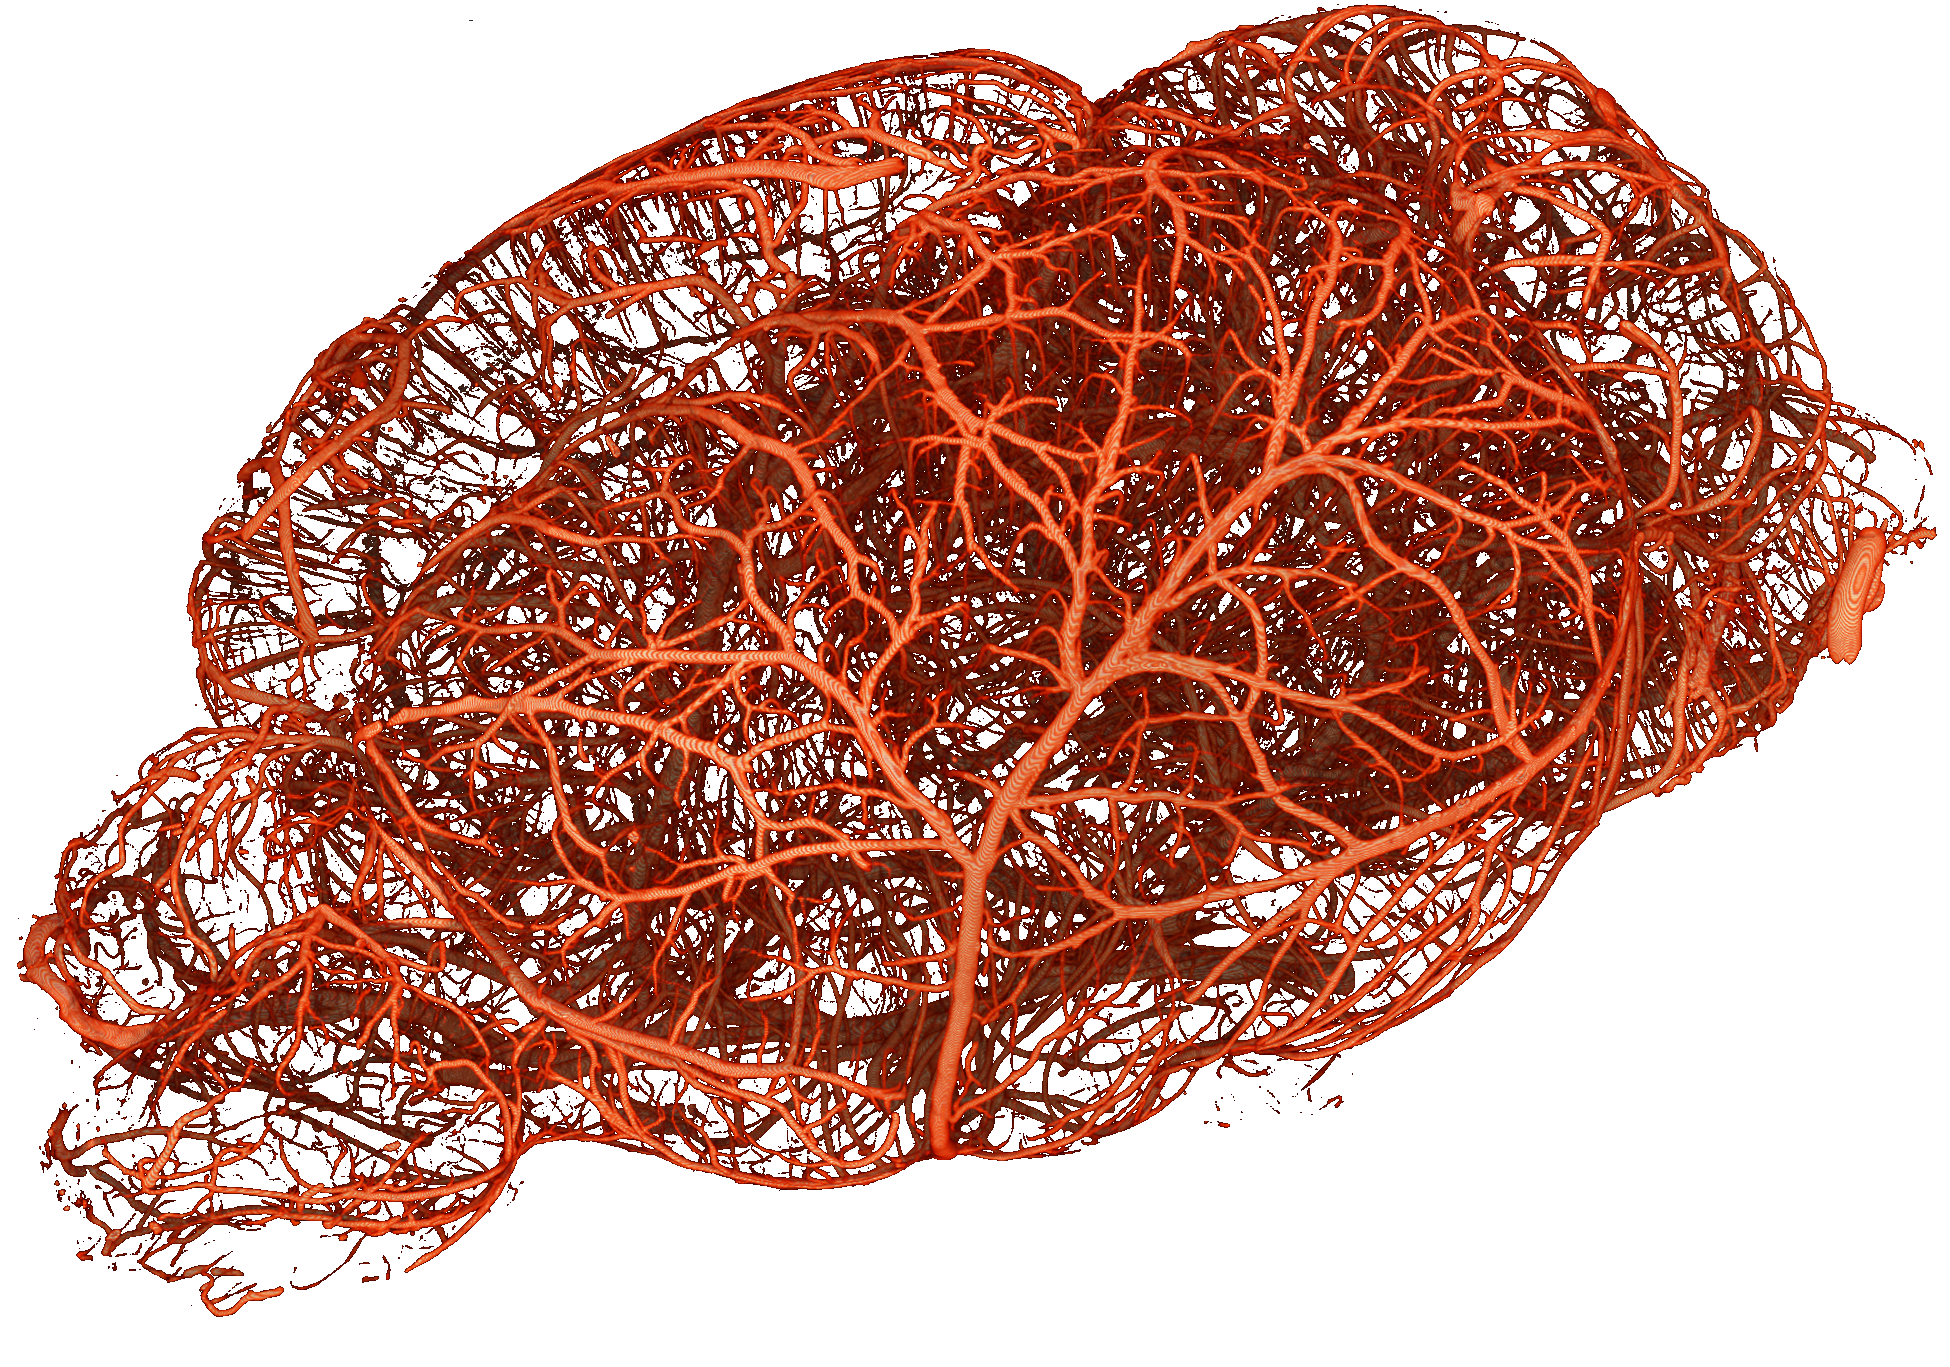
\includegraphics[width=\imagewidth]{img/Ebene_25}};
            % 1949px = 20.0mm > 100px = 1026um > 49px = 500um, 10px = 100um
            %\draw[|-|,blue,thick] (39,1222) -- (1722,239) node [sloped,midway,above,fill=white,semitransparent,text opacity=1] {\SI{20.0}{\milli\meter} (1949px) TEMPORARY!};
            \draw[|-| ] (\x,\y) -- (\x+97,\y) node [midway,above] {\SI{1}{\milli\meter}};
            \node [anchor=center] (cb) at (2200,300) {Cerebellum};
            \draw [thick] (cb.west) to [out=-180, in=0] (1482,144);
            \node [anchor=center] (bs) at (2200,500) {Brain stem};
            \draw [thick] (bs.south) to [out=-90, in=-45] (1705,725);
            \node [anchor=center, text width=2cm, align=center] (ob) at (-150,1200) {Olfactory bulbs};
            \draw [thick] (ob.north) to [out=90, in=180] (210,880);
            \draw [thick] (ob.north) to [out=90, in=180] (298,1116);
        \end{tikzpicture}
        \caption{Visualization of a tomographic scan of a \uaf-filled mouse brain. Will be important later on with \emph{Grenoble} brains.}%
    \end{figure}%       
\end{frame}

\section{Assessing tumor/metastasis load in lungs}
\begin{frame}{Tumor metastasis}
	\begin{itemize}
		\item Assessing tumor load in lungs
		\item KP-TNIK mice
		\item Stereology
	\end{itemize}
\end{frame}

\renewcommand{\imsize}{0.27\linewidth}  
\begin{frame}{Tumor load in lungs, KP-TNIK mice. Top: KO, bottom: WT}
    \pgfmathsetlength{\imagewidth}{\imsize}%
    \pgfmathsetlength{\imagescale}{\imagewidth/800}%
    \def\x{494}% scalebar-x starting at golden ratio of image width of 800px = 494
    \def\y{720}% scalebar-y at 90% of image height of 800px = 720
	\begin{tikzpicture}[x=\imagescale,y=-\imagescale]
		\node[anchor=north west, inner sep=0pt, outer sep=0pt] at (0,0) {\includegraphics[width=\imagewidth]{../../Documents/Collaborations/DKF_Lung/Overview/{{MAX_--11}}}};
		% 800px = 16.0mm > 100px = 2000um > 25px = 500um, 5px = 100um
		%\draw[|-|,blue,thick] (0,400) -- (800,400) node [sloped,midway,above,fill=white,semitransparent,text opacity=1] {\SI{16.0}{\milli\meter} (800px) TEMPORARY!};
		\draw[|-|] (\x,\y) -- (\x+250,\y) node [midway,above] {\SI{5}{\milli\meter}};
	\end{tikzpicture}%
	\hfill%
	\begin{tikzpicture}[x=\imagescale,y=-\imagescale]
		\node[anchor=north west, inner sep=0pt, outer sep=0pt] at (0,0) {\includegraphics[width=\imagewidth]{../../Documents/Collaborations/DKF_Lung/Overview/{{MAX_--12}}}};
		\draw[|-|] (\x,\y) -- (\x+250,\y) node [midway,above] {\SI{5}{\milli\meter}};
	\end{tikzpicture}%
	\hfill%
	\begin{tikzpicture}[x=\imagescale,y=-\imagescale]
		\node[anchor=north west, inner sep=0pt, outer sep=0pt] at (0,0) {\includegraphics[width=\imagewidth]{../../Documents/Collaborations/DKF_Lung/Overview/{{MAX_--13}}}};
		\draw[|-|] (\x,\y) -- (\x+250,\y) node [midway,above] {\SI{5}{\milli\meter}};
	\end{tikzpicture}\\%
	\begin{tikzpicture}[x=\imagescale,y=-\imagescale]
		\node[anchor=north west, inner sep=0pt, outer sep=0pt] at (0,0) {\includegraphics[width=\imagewidth]{../../Documents/Collaborations/DKF_Lung/Overview/{{MAX_wt11}}}};
		\draw[|-|] (\x,\y) -- (\x+250,\y) node [midway,above] {\SI{5}{\milli\meter}};
	\end{tikzpicture}%
    \hfill%    
	\begin{tikzpicture}[x=\imagescale,y=-\imagescale]
		\node[anchor=north west, inner sep=0pt, outer sep=0pt] at (0,0) {\includegraphics[width=\imagewidth]{../../Documents/Collaborations/DKF_Lung/Overview/{{MAX_wt12}}}};
		\draw[|-|] (\x,\y) -- (\x+250,\y) node [midway,above] {\SI{5}{\milli\meter}};
	\end{tikzpicture}%
    \hfill%    
	\begin{tikzpicture}[x=\imagescale,y=-\imagescale]
		\node[anchor=north west, inner sep=0pt, outer sep=0pt] at (0,0) {\includegraphics[width=\imagewidth]{../../Documents/Collaborations/DKF_Lung/Overview/{{MAX_wt13}}}};
		\draw[|-|] (\x,\y) -- (\x+250,\y) node [midway,above] {\SI{5}{\milli\meter}};
	\end{tikzpicture}%
\end{frame}

\begin{frame}{Tumor load in lungs, KP-TNIK mice. Top: KO, bottom: WT}
	\renewcommand{\imsize}{\linewidth}  
	\animategraphics[palindrome,width=\imsize]{12}{../../Documents/Collaborations/DKF_Lung/movieframes/out-}{001}{255}
\end{frame}

\section{Multimodal imaging: \uct and 3View, correlated}
\begin{frame}{Overview scan with \SI{20}{\micro\meter} pixel size}
    \renewcommand{\imsize}{0.5\linewidth}  
	\pgfmathsetlength{\imagewidth}{\imsize}%
	\pgfmathsetlength{\imagescale}{\imagewidth/864}%
	\def\x{534}% scalebar-x starting at golden ratio of image width of 864px = 534
	\def\y{723}% scalebar-y at 90% of image height of 803px = 723
	\begin{tikzpicture}[x=\imagescale,y=-\imagescale, spy using outlines={rectangle, magnification=\mag, size=\size, connect spies}]
		\node[anchor=north west, inner sep=0pt, outer sep=0pt] at (0,0) {
			\animategraphics[palindrome, width=\imsize]{24}{./img/movie_tumor_20um/image}{3503}{4037}
			};
		% 592px = 19.723mm > 100px = 3331um > 15px = 500um, 3px = 100um
		%\draw[|-|,blue,thick] (194,615) -- (685,284) node [sloped,midway,above,fill=white,semitransparent,text opacity=1] {\SI{19.723}{\milli\meter} (592px) TEMPORARY!};
		\draw[|-|] (\x,\y) -- (\x+300,\y) node [midway,above] {\SI{1}{\centi\meter}};
		%\draw[color=red, anchor=south west] (0,803) node [fill=white, semitransparent] {Legend} node {Legend};
	\end{tikzpicture}%
\end{frame}

\begin{frame}{Overview, Detail and 3View}
	\renewcommand{\imsize}{0.25\linewidth}
	\includegraphics[width=\imsize]{../../Documents/ProgressReports/2016.10-Fibrosis/img/Mouse_Tumor_IR_rec00001610_scalebar}
	\pause
	\includegraphics[width=\imsize]{../../Documents/ProgressReports/2016.10-Fibrosis/img/uct_Cube_scalebar}
	\pause
	\includegraphics[width=\imsize]{../../Documents/ProgressReports/2016.10-Fibrosis/img/3View_Overview_scalebar.jpg}
	\pause
	\includegraphics[width=\imsize]{../../Documents/ProgressReports/2016.10-Fibrosis/img/3View_Detail_scalebar.jpg}	
	\note{%
		\begin{itemize}
			\item 3View
			\begin{itemize}
				\item Slice 297/500 from each of the datasets (ROI00 and ROI01)
				\item Manually registered with 6 points and Plugins > Registration > Moving least squares
				\item Saved on anadata/djonov > uct > Mouse\_Lung\_Metastasis > Valentin
			\end{itemize}
			\item \uct
				\begin{itemize}
					\item Mouse\_Tumor\_Cube
					\item Mouse\_Tumor\_Cube\_rec00002639 registered with slice 297 of 3View\_Registration.tif
				\end{itemize}
		\end{itemize}
	}
\end{frame}

\begin{frame}{Overview, Detail and 3View}
	\renewcommand{\imsize}{0.5\linewidth}
	\includegraphics<1>[width=\imsize]{../../Documents/ProgressReports/2016.10-Fibrosis/img/3View_Overview_scalebar}
	\includegraphics<2>[width=\imsize]{../../Documents/ProgressReports/2016.10-Fibrosis/img/3View_Registration_scalebar}
	\includegraphics<3>[width=\imsize]{../../Documents/ProgressReports/2016.10-Fibrosis/img/uCT_Cube_with_3View_Registration_Average_scalebar.jpg}
\end{frame}

\section{Brain tumors}
\begin{frame}{Brain tumor radiation treatment}
    \begin{itemize}
        \item Induced tumors in rat brains
        \item Microbeam and broadbeam treatment vs.\ control
        \item \uaf-filled brain vasculature
        \item Nondestructive extraction of
        \begin{itemize}
            \item Vessel to tumor volume ratio
            \item Vessel surface
            \item Intra-tumoral microvessel density (IMD, \cite{Hasan2002})
        \end{itemize}
    \end{itemize}
\end{frame}

\renewcommand{\imsize}{0.9\linewidth}	
\begin{frame}{vessel volume ratio}
    \includegraphics[width=\imsize]{../../Documents/Brain-Grenoble/fig/vessel_ratio_violin}
\end{frame}

\begin{frame}{vessel surface}
    \includegraphics[width=\imsize]{../../Documents/Brain-Grenoble/fig/vessel_surface_per_tumor_volume}
\end{frame}

\begin{frame}{imd}
    \includegraphics[width=\imsize]{../../Documents/Brain-Grenoble/fig/slice_imd}
\end{frame}

\begin{frame}{Thanks}
	\begin{itemize}
		\item Topographic and clinical Anatomy
		\item SNF
		\pause
		\item You, for listening
		\pause
		\item Questions?
	\end{itemize}
\end{frame}

\begin{frame}{References}
    \renewcommand*{\bibfont}{\tiny}
    \printbibliography
\end{frame}

\end{document}